%-------------
%---| Q02 |---
\addcontentsline{toc}{section}{Questão 01 ref: P02}
\begin{prob}[ref: P02]
	Quando o Sol se põe, decorrem aproximadamente 2 minutos entre o instante em que o disco solar encosta no horizonte e sua ocultação completa. A partir deste dado, estime o diâmetro angular aparente do Sol visto da Terra, em graus.
\end{prob}

\begin{sol}
	\textcolor {teal} {
		Assumindo um dia em que o sol demora 12 horas entre o nascer e o ocaso temos que
		\begin{align}
			\frac{\theta_{sol}}{180^{\circ}}&=\frac{2min}{720min}\quad \therefore\quad\theta_{sol}=0,5^{\circ}			
		\end{align}
	}
\end{sol}
%-------------
%---| Q03 |---
\addcontentsline{toc}{section}{Questão 02 ref: P03}
\begin{prob}[ref: P03]
	No dia do solstício de verão (o mais longo do ano), na cidade de Siena, ao meio dia, os raios solares eram exatamente verticais. Neste dia e hora, Eratóstenes mediu a sombra projetada por uma
	estaca vertical na cidade de Alexandria e descobriu que ela tinha um oitavo da altura da estaca. Além disso, a distância entre as duas cidades já era conhecida como 5000 estádios (1 estádio aproximadamente 157 metros). Com estes dados, calcule o raio da Terra.
\end{prob}

\begin{sol}
	\textcolor{teal} {
		Sabe-se que o comprimento $C$ de uma circunferência de raio $R$ é dado por:
		\begin{align}
			C&=2\pi R
			\label{eq:comprimento-circ}
		\end{align}
		Da eq. \eqref{eq:comprimento-circ} é fácil de ver que se soubermos $C$, então $R$ é imediato. Outro ponto a se considerar é o comprimento do arco de um setor da mesma circunferência dado por
		\begin{align}
			c&=\alpha R
			\label{eq:comprimento-setor}
		\end{align}
		estas grandezas são proporcionais de modo que
		\begin{align}
			\frac{C}{c}&=\frac{2\pi R}{\alpha R}
		\end{align}
		logo
		\begin{align}
			C&=c\left(\frac{2\pi}{\alpha}\right)
		\end{align}
		no caso:
		\begin{itemize}
			\item C é o comprimento da circunferência terrestre;
			\item c é o comprimento do arco de circuferência, que vai de Siena a Alexandria;
			\item $\alpha$ é o ângulo entre as duas cidades medido a partir do centro da terra, essencialmente o mesmo ângulo que o raio de sol incide na estaca em Alexndria. 
		\end{itemize}
		Para determinar $\alpha$ (em Alexandria), basta fazer
		\begin{align}
			\tan \alpha&=\frac{h/8}{h}=\frac{1}{8} \nonumber \\
			\alpha&=\arctan\left(\frac{1}{8}\right) \nonumber \\
			\alpha&=7,13^{\circ}
		\end{align}
		Assim
		\begin{align}
			C=5000\times 157m\left(\frac{360^{\circ}}{7,13^{\circ}}\right)=3,96\times 10^{7}m
		\end{align}
		e por fim
		\begin{align}
			R=\frac{C}{2\pi}=6,30\times 10^{6}m
		\end{align}
	}
\end{sol}
%-------------
%---| Q05 |---
\addcontentsline{toc}{section}{Questão 03 ref: P05}
\begin{prob}[ref: P05]
	No século III A.C, o astrônomo Aristarco de Samos estimou a razão $d_{S}/d_{L}$ entre a distância $d_{S}$ da Terra ao Sol e distância $d_{L}$ da Terra à Lua medindo o ângulo $\theta$ entre as retas Terra-Sol e Terra-Lua. O valor obtido foi $\theta=87^{\circ}$.
	\begin{enumerate}[label=\alph *)]
		\item Encontre a estimativa de Aristarco para $d_{S}/d_{L}$.
		\item Com base nos valores atualmente conhecidos, $d_{S}/d_{L}\sim 389$. Determine o valor atual de $\theta$ e argumente porque o método de Aristarco não produz um bom resultado.
	\end{enumerate}
\end{prob}

\begin{sol}
	\textcolor{teal} {
		\begin{enumerate}[label=\alph *)]
			\item Dado que
			\begin{align}
				\cos \theta&=\frac{d_L}{d_S} \nonumber \\
				\sec \theta&=\frac{d_S}{d_L}
			\end{align}
			logo, a estimativa de Aristarco para a razão $d_S/d_L$ é simplesmente
			\begin{align}
				\frac{d_S}{d_L}&=\sec 89^{\circ}=19,1
			\end{align}
			\item Para os valores atuais tem-se
			\begin{align}
				\sec \theta&=389 \nonumber \\
				\theta&=\sec^{-1}389\approx 89,9^{\circ}				
			\end{align}
			Ainda que o ângulo obtido por Aristarco difere cerca de $3^{\circ}$ do valor de ângulo atual, a razão para $d_S/d_L$ encontrada por Aristarco é da ordem de 20 vezes menor que os resultados atuais, isso de fato deve requerer um instrumento de medida de ângulos altamente preciso, o que evidentemente não existia naquela época, um outro ponto a se destacar é que a execução deste experimento requer alto grau de acurácia do experimentador para identificar o momento exato em que a metade da lua está completamente iluminada, um dia antes ou depois da observação pode alterar minimamente o valor de ângulo observado produzindo assim, alta discrepância na razão $d_S/d_L$. Por fim, há ainda de se considerar se Aristarco conhecia os trabalhos de Eratóstenes no que diz respeito a medida do raio da terra, visto que supostamente a medida de ângulo obtida por ele, foi realizada na superfíce do planeta e não em seu centro, como inlustra a figura do exercício, medidas mais atuais \cite{BERTUOLA2016} apontam para uma diferença de $0^{\circ}3^{\prime }0^{\prime \prime}$, diferença pequena mas que pode contribuir para uma melhor aproximação.
		\end{enumerate}
	}
\end{sol}
%-------------
%---| Q09 |---
\addcontentsline{toc}{section}{Questão 04 ref: P09}
\begin{prob}[ref: P09]
	Desenhe um circulo representando a esfera celeste para um observador localizado em um lugar
	de latitude $20^{\circ}N$. Nesse círculo marque:
	\begin{enumerate}[label=\alph *)]
		\item A localização do zênite
		\item A localização do pólo elevado, e o ângulo que ele faz com o horizonte
		\item O plano do equador
		\item O plano do horizonte, com os pontos cardeais $N,S,L,O$
		\item A calota das estrelas circumpolares visíveis
		\item O círculo diurno de uma estrela de declinação $\delta=+40^{\circ}$
	\end{enumerate}
\end{prob}
\newpage
\begin{sol}
	\textcolor{teal} {
		\begin{figure}[!ht]
			\centering
			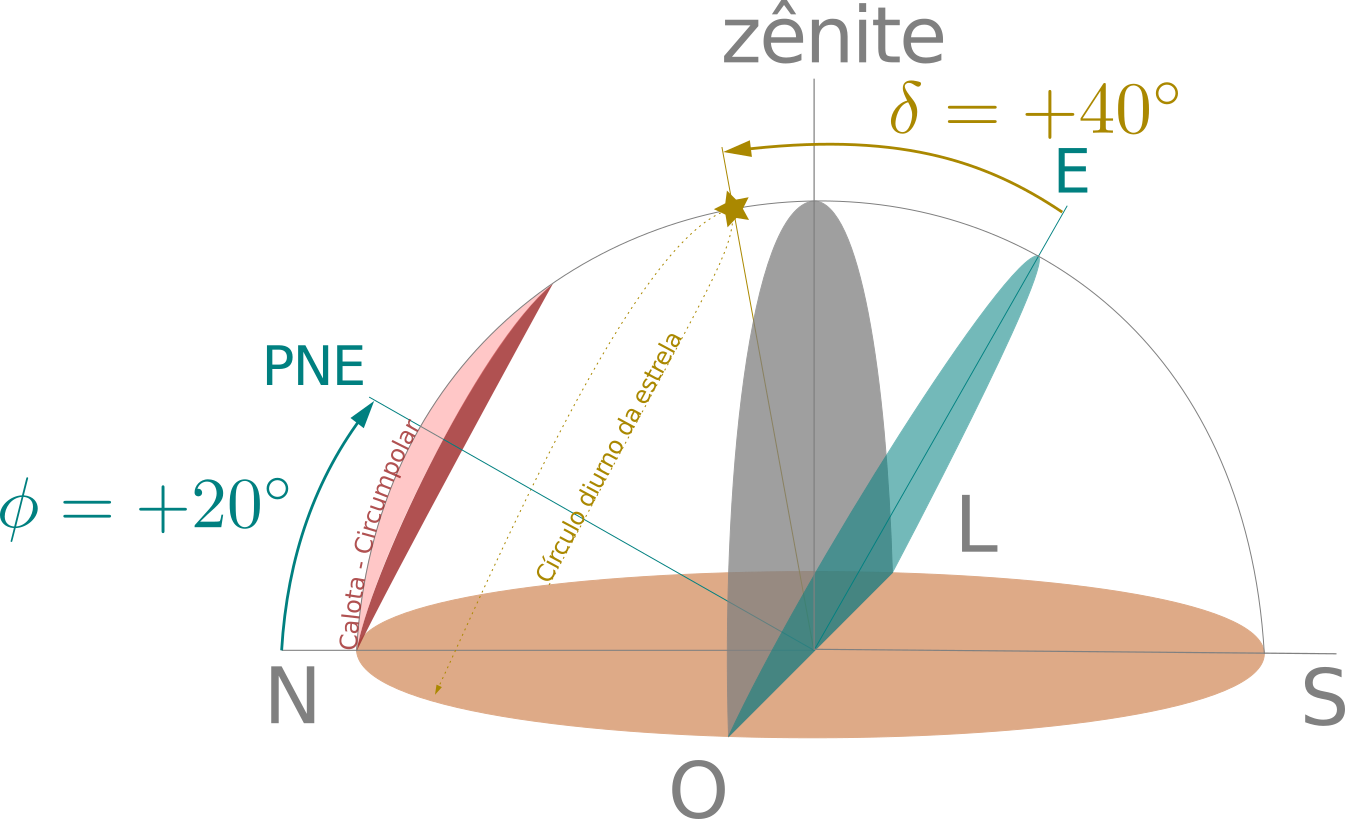
\includegraphics[width=.75\linewidth]{fig/fig-q4.png}
			\caption{Esquema representativo da esfera celeste para um observador localizado numa latitude $\phi=\degree{20}{N}$}
			\label{fig:fig-ex4}
		\end{figure}
	}
\end{sol}
%-------------
%---| Q015 |---
\addcontentsline{toc}{section}{Questão 05 ref: P15}
\begin{prob}[ref: P15]
	Encontre uma relação entre o módulo da latitude do observador e o módulo da declinação de
	uma estrela para que esta seja circumpolar.	
\end{prob}

\begin{sol}
	\textcolor{teal} {
		A figura \eqref{fig:ex15} representa um diagrama do plano meridiano de uma estrela com declinação $\delta$ em um local do hemisfério Norte de latitude $\phi$ 
		\begin{figure}[!ht]			
			\centering
			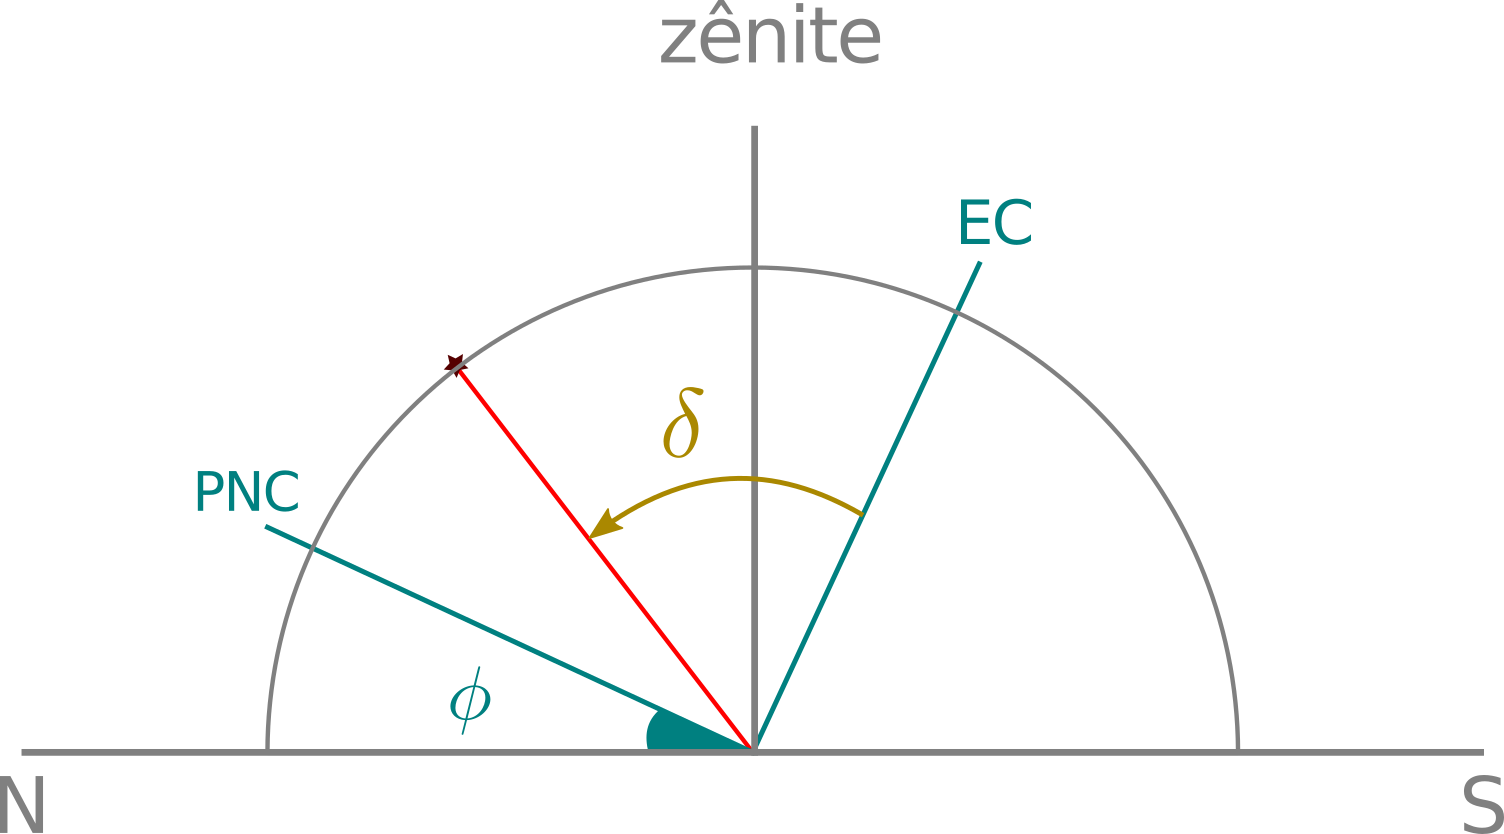
\includegraphics[width=0.5\linewidth]{fig/fig-q15.png}			
			\caption{Diagrama do plano meridiano representando uma estrela para um observador localizado no hemisfério Norte}
			\label{fig:ex15}
		\end{figure}
	}
	
	\textcolor{teal} {
		A condição para que uma estrela de declinação $\delta$ seja circumpolar, é que ela deve pertencer à região da calota esférica de raio igual à latitude local $\phi$ e centro no pólo elevado, o que neste caso é o pólo Norte. Da figura \eqref{fig:ex15}, tiramos que se $\delta$ for maior que $\degree{90}{}-\phi$ (uma vez que o pólo elevado reside na bissetriz da calota polar e forma um ângulo reto com o Equador Celeste $EC$) a estrela de declinação $\delta$ é circumpolar. Portanto, para um observador localizado no hemisfério Norte é suficiente que
		\begin{align}
			\delta&\geq \degree{90}{}-\phi
			\label{eq:circP-HN}
		\end{align}
		De forma análoga e observando que para um observador situado no hemisfério Sul $\delta<0$ e $\phi<0$ tem-se a seguinte relação
		\begin{align}
			\delta&\leq -(\degree{90}{}+\phi)
			\label{eq:circP-HS}
		\end{align}
		generalizando o que encontramos nas equações \eqref{eq:circP-HN} e \eqref{eq:circP-HS}, além de notar que
		\begin{align}
			\left|\phi \right|&=\left\{\begin{matrix}
				\phi & se, & \phi\geq0  \\
				-\phi & se,& \phi<0  \\
				\end{matrix}\right.
		\end{align}
		\begin{align}
			\left(\degree{90}{}-|\phi|\right)-&\geq\delta\geq\degree{90}{}-|\phi| 
		\end{align}
		ou ainda
		\begin{align}
			|\delta|&\geq\degree{90}{}-|\phi|
		\end{align}
	}			
\end{sol}
%-------------
%---| Q017 |---
\addcontentsline{toc}{section}{Questão 06 ref: P17}
\begin{prob}[ref: P17]
	Mostre que o dia sideral é cerca de 4 minutos mais curto que o dia solar. Justifique com cálculos
	e desenhos.
\end{prob}

\begin{sol}
	\textcolor{teal} { 
		O dia sideral é definido como duas passagens consecutivas do ponto vernal $\gamma$ pelo meridiano local. Por decorrência do movimento de translação da Terra em torno do Sol e da distância da Terra em relação ao Sol ser muito menor se comparado à distância da Terra ao primeiro ponto de Áries (ponto vernal - $\gamma$), a Terra percorre o equivalente a \degree{0,986}{} por dia a mais para se alinhar novamente ao Sol, completando assim o dia solar. Esta pequena diferença ângular transformada em horas resulta em
		\begin{align}
			\frac{\degree{360}{}}{\degree{0,986}{}}&=\frac{24h}{x}\nonumber \\
			x&=\frac{\left(24h\right)\left(\degree{0,986}{}\right)}{\degree{360}{}}\nonumber \\
			x&=0,065733\left(60min\right)\nonumber \\
			x&=3,944min
		\end{align}
		e é o tempo necessário para a Terra completar um dia solar, após ter completado um dia sideal.
	}
\end{sol}
%-------------
%---| Q19 |---
\addcontentsline{toc}{section}{Questão 07 ref: P19}
\begin{prob}[ref: P19]
	A Lua, vista da Terra, se movimenta em relação ao fundo de estrelas a uma taxa de $\degree{13}{}10^{\prime}35^{\prime \prime}$ para leste por dia. Qual a duração do "dia lunar", isto é, o intervalo de tempo decorrido entre duas culminações sucessivas da Lua? Justifique com cálculos e desenhos.
\end{prob}

\begin{sol}
	\textcolor{teal} {
		Considerando que o movimento aparente da Lua com relação as estrelas fixas, dá-se a uma taxa de $D_{L}=\degree{13}{}10^{\prime}35^{\prime \prime}$ para leste a cada dia $\theta_{d}=\degree{360}{}$ (fato devido ao movimento de translação da Lua em torno da Terra), e que o Sol por sua vez, executa o movimento aparente de \degree{1}{} para leste a cada dia (fato devido ao movimento de translação da Terra em torno do Sol) \cite{ASTRN&ASTRFIS:2004}, então o movimento aparente relativo entre o sistema Sol-Lua é de $(\degree{13}{}10^{\prime}35^{\prime \prime}-\degree{1}{})=\degree{12}{}10^{\prime}35^{\prime \prime}/dia$ ou $D^{\prime}_{L}\approx \degree{12}{}/dia$. Sendo assim. O período de atraso da Lua $T_L$ a cada dia é calculado por
		\begin{align}
			T_{L}&=\frac{D^{\prime}_{L}}{\theta_{d}}\approx \frac{\degree{12}{}}{\degree{360}{}}\nonumber \\
			T_{L}&\approx 0,033823
		\end{align}
		convertendo para o formato $hh:mm:ss$, temos que a Lua sofre um atraso de
		\begin{align}
			T_{L}&\approx 0,033823\times 24h\times 60min \nonumber \\
			T_{L}&\approx 48min
		\end{align}
		Logo, o dia lunar pode ser determinado considerando o tempo entre duas passagens consecutivas da Lua pelo meridiano superior do local acrescido do seu período de atraso por dia
		\begin{align}
			24h+T_{L}&=24h48min
		\end{align}
	}
\end{sol}
%-------------
%---| Q20 |---
\addcontentsline{toc}{section}{Questão 08 ref: P20}
\begin{prob}[ref: P20]
	O mês lunar (tempo para repetição de uma mesma fase) é de 29,53 dias. Calcular a duração do
	mês sideral (tempo para dar uma volta completa em torno da Terra). Justifique com cálculos e desenhos.
\end{prob}

\begin{sol}	
	\textcolor{teal} {
		Levando-se em considerção que o período necessário para que ocorra duas fases consecutivas da Lua é de $t_2=29,53$ dias. Da figura \eqref{fig:fig-ex20} é possível verificar que estas configurações ocorrem após a Lua percorrer um ângulo tal que $\beta_2=\beta_{1}+\theta$ no intervalo de tempo considerado. O ângulo $\beta_{1}$ é conhecido, precisamos saber quanto vale o ângulo $\theta$ para saber a diferença de tempo necessário para que ocorra a configuração intermediária $t_{1}$ como mostra a figura abaixo
		\begin{figure}[!ht]
			\centering
			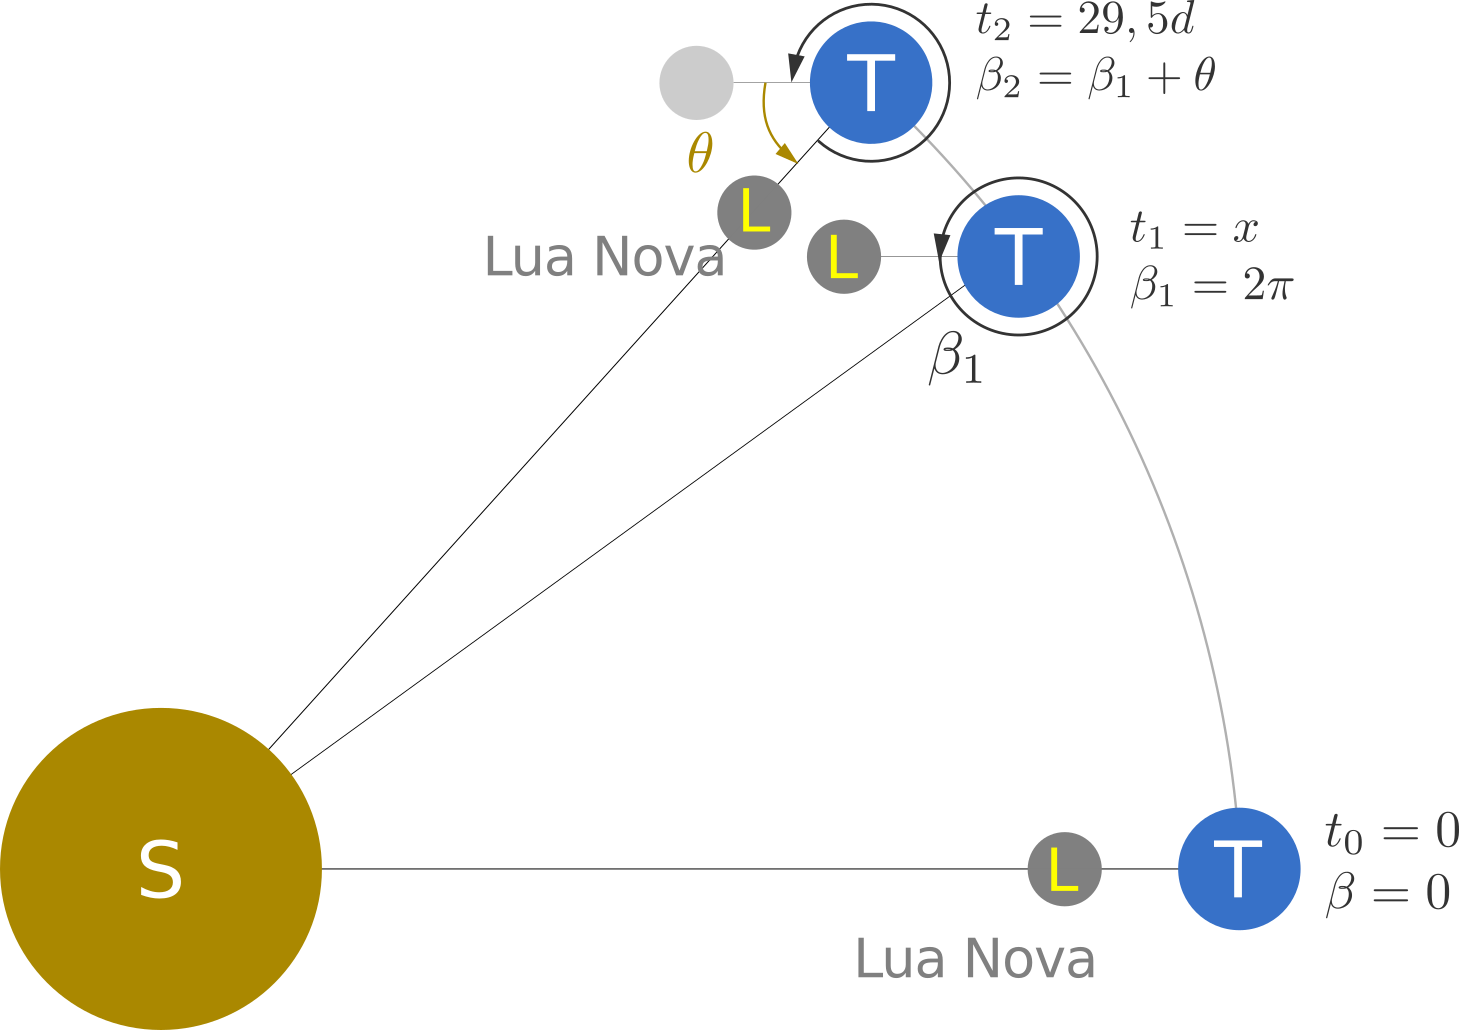
\includegraphics[width=.5\linewidth]{fig/fig-q20.png}
			\caption{Esquema representativo (e exagerado) do sistema Sol-Lua-Terra entre duas fases lunares $t_0$ e $t_2$ consecutivas}
			\label{fig:fig-ex20}
		\end{figure}		
	}
	\newpage
	\textcolor{teal} {
		Ora, sabemos que a terra devido ao seu movimento de translação, desloca-se $\degree{0,986}{}$ a mais da sua rotação para alinhar-se completamente ao Sol novamente completando assim 1 dia solar, sabemos também que as fases da Lua Nova só podem ocorrer em dias solares haja visto que estes fenômenos ocorrem sempre em conjunto com a conjunção destes astros, portanto o período de 29,53 dias decorridos no mês lunar deve corresponder, essencialmente, a 29,53 dias solares. Dito isso, temos que
		\begin{align}
			\theta&=29,53\times \degree{0,986}{}=\degree{29,11658}{}
		\end{align}
		sendo assim
		\begin{align}
			\beta_{2}&=\degree{360}{}+\degree{29,11658}{}=\degree{389,11658}{}
		\end{align}
		Logo, a duração do mês sideral lunar $t_1$ é
		\begin{align}
			\frac{\degree{389,11658}{}}{\degree{360}{}}&=\frac{29,53d}{t_1}\nonumber \\
			t_{1}&=27,32035 \ dias
		\end{align}
	}
\end{sol}
%-------------
%---| Q21 |---
\newpage
\addcontentsline{toc}{section}{Questão 09 ref: P21}
\begin{prob}[ref: P21]
	As estações do ano ocorrem devido à mudança na quantidade de radiação solar absorvida pela Terra. Estime a razão das insolações na cidade de Porto Alegre (latitude: \degree{30}{S}):
	\begin{enumerate}[label=\alph *)]
		\item $\frac{I_v}{I_i}$ ao meio dia (maior altura do Sol), onde $I_v$ é a insoloação no solstício de verão e $I_i$ a insoloação no solstício de inverno.
		\item $\frac{I_p}{I_a}$, onde $I_p$ é a insoloação quando a Terra está no periélio e $I_a$ a insoloação quando a Terra está no afélio.
		\item comparando estes resultados, qual efeito é mais relevante para as estações do ano?
	\end{enumerate}
\end{prob}

\begin{sol}
	\textcolor{teal} {
		\begin{enumerate}[label=\alph *)]
			\item Ao meio dia em Porto Alegre no verão o Sol incide sobre a eclíptica a um ângulo de $\delta_{V}=\degree{+23,5}{}$ longo
			\begin{align}
				\theta_{V}&=\left(\degree{90-\phi}{}\right)+\delta_{V}\nonumber \\
				\theta_{V}&=\degree{83,5}{}
			\end{align}
			e no inverno o Sol incide sobre a eclíptica a um ângulo de $\delta_{I}=\degree{-23,5}{}$ e assim
			\begin{align}
				\theta_{I}&=\left(\degree{90}{}\right)-\delta_{I}\nonumber \\
				\theta_{I}&=\degree{36,5}{}
			\end{align}
			Para este caso a insolação fica
			\begin{align}
				\frac{I_V}{I_I}&=\frac{\sen\theta_V}{\sen\theta_I}				
			\end{align}
			logo
			\begin{align}
				I_V&=\frac{0,99}{0,59}I_I=1,66I_I
			\end{align}
			ou seja, no verão a quantidade de radiação solar absorvida pela Terra é 66\% a mais que no inverno.
			\item Sendo a distância entre a Terra e o Sol no periélio $R_{p}=147\times 10^{6}km$ e no afélio $R_{a}=152\times 10^{6}km$, a razão entre as insolações $I_p$ e $I_a$ para estes casos é dada por
			\begin{align}
				\frac{I_p}{I_a}&=\left(\frac{R_a}{R_p}\right)^2
			\end{align}
			substituindo temos
			\begin{align}
				\frac{I_p}{I_a}&=\left(\frac{147\times 10^{6}km}{152\times 10^{6}km}\right)^2
			\end{align}
			o que resulta em
			\begin{align}
				I_p&=0,94I_a
			\end{align}
			\item Dos resultados dos itens (a) e (b) temos que a maior contribuição para a ocorrência das estações do ano, decorre da inclinação da eclíptica visto que este fato contribui significantemente mais para a absorção da energia solar pela Terra (66\%) do que a proximidade da Terra ao Sol como ocorre nos periélios e afélios onde a contribuição é cerca de $|0,94-1|=0,06$ i.e. 6\% a mais no periélio do que no afélio.
		\end{enumerate}
	}
\end{sol}
%-------------
%---| Q22 |---
\addcontentsline{toc}{section}{Questão 10 ref: P22}
\begin{prob}[ref: P22]
	Calcule o comprimento da sombra da Terra, considerando–se a distância média Terra – Sol e sabendo que o raio da Terra vale $6370 km$ e o raio do Sol $696000 km$.
\end{prob}

\begin{sol}
	\textcolor{teal} {
		vamos calcular primero a distância média Terra-Sol ($D_{\oplus \odot }$) usando os valores da distância no periélio $147\times 10^{6}km$ e no afélio $152\times 10^{6}km$
		\begin{align}
			D_{\oplus \odot}&=\frac{\left(147+152\right)\times10^{6}km}{2}=149,5\times10^{6}km
		\end{align}
		Por fim, o comprimento da sombra da Terra é
		\begin{align}
			L&=\frac{R^{\prime}D_{\oplus \odot}}{R-R^{\prime}}\nonumber \\
			L&=\frac{\left(6,37\times10^{3}km\right)\left(1,495\times10^{8}km\right)}{6,96\times10^{5}km-6,37\times10^{3}km}
		\end{align}
		ou seja
		\begin{align}
			L&=1,389\times10^{6}km
		\end{align}
	}
\end{sol}